% !TeX encoding = UTF-8
% !TeX spellcheck = en_US
% !TeX TXS-program:bibliography = biber -l zh__pinyin --output-safechars %
%% !TeX TS-program = xelatex

\documentclass[a4paper,10pt]{article}

\newcommand{\hwNumber}{3}

% to be `\input` in subfolders,
% ... therefore the path should be relative to subfolders.

\usepackage[UTF8
	,heading=false
	,scheme=plain % English Document
]{ctex}
\usepackage{indentfirst}

\input{../.modules/basics/macros.tex}
\input{../.modules/preamble_base.tex}
\input{../.modules/preamble_notes.tex}

\newcommand{\legacyReference}{{
	\clearpage\par
	\quad\clearpage
	\renewcommand{\midquote}{\textbf{PAST WORK, AS TEMPLATE}}
	\newparagraph
}}

% Settings
\counterwithout{equation}{section}
\mathtoolsset{showonlyrefs=false}
%\DeclareTextFontCommand{\textbf}{\sffamily}
\renewcommand{\midquote}{\quad}
\resizegathersetup{equations=false}

% Spacing
\geometry{footnotesep=2\baselineskip} % pre footnote split
\setlength{\parskip}{.5\baselineskip}
\renewcommand{\baselinestretch}{1.15}

%Title
	\posttitle{
		\hfill\Large\ccbyncsajp
		\par\end{flushleft}%
		\vspace*{-.7ex}\hrule%
	}
	\preauthor{\vspace{-1.5ex}%
		\flushleft\itshape%
	}
	\postauthor{\hfill}
	\predate{\noindent\ttfamily Compiled @ }
	\postdate{\vspace{.5ex}}

	\title{Finite Temperature Field Theory \textnumero\hwNumber}
	\author{\signature Bryan}
	\date{\today}

% List
	\setlist*{
		listparindent=\parindent
		,labelindent=\parindent
		,parsep=\parskip
		,itemsep=1.2\parskip
	}
	\setlist*[enumerate,1]{
		align=left
		,label=\fbox{\textbf{\arabic*}}
		,itemsep=.5\baselineskip
	}

\input{../.modules/basics/biblatex.tex}

%%% ID: sensitive, do NOT publish!
%\InputIfFileExists{../id.tex}{}{}

\begin{document}
\maketitle
\pagestyle{headings}
\pagenumbering{arabic}
\thispagestyle{empty}

\vspace*{-1.5\baselineskip}

\subsection*{QCD Partition Function at $\order{g^2}$}
	\begin{center}
		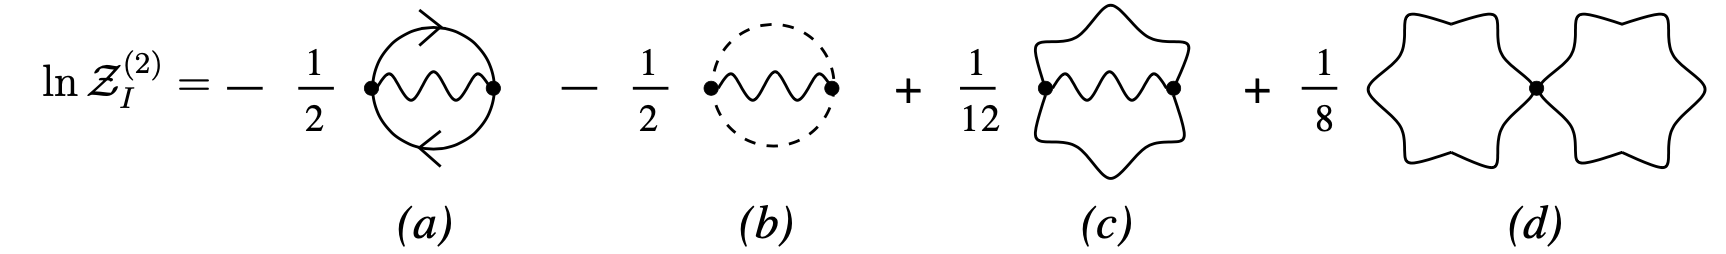
\includegraphics[width=.9\linewidth]{qcd_partition.png}
	\end{center}
	\vspace{-.5\baselineskip}
	\begin{equation}
		\ln \mcal{Z}^{(2)}_I
		= \ln \mcal{Z}^{(a)}
			+ \ln \mcal{Z}^{(b)}
			+ \ln \mcal{Z}^{(c)}
			+ \ln \mcal{Z}^{(d)}
	\end{equation}
	
	The contribution of (a) is given by:
	\begin{equation}
		\ln \mcal{Z}^{(a)}
		= \frac{1}{2!}\,(-1)^1
			\frac{T}{V} \sum_k\,
			\frac{T}{V} \sum_p\,
				\Tr \pqty\Big{
					S(k)\,(g\gamma^\nu T^b)\,
					S(p)\,(g\gamma^\mu T^a)
				}\,
				\pqty{
					\frac{V}{T}
				}\,\delta_{ab}\,
				\Delta_{\mu\nu}(p - k)
	\end{equation}
	Here the trace goes over spinor, color and flavor indices. 
	$S(k)$ is the quark propagator, with suppressed spinor, color and flavor indices, while $\delta_{ab}\,\Delta_{\mu\nu}$ is the gluon propagator, where $a, b$ are adjoint indices; each vertex contributes a $(g\gamma^\mu T^a)$ factor. 
	
	In our convention, $k = (\omega_n, \vb{k})$ stands for the Euclidean 4-momentum with $\omega_n$: the discrete Matsubara frequency. Each $\sum_k$ comes with a factor $\frac{T}{V}$ while each momentum space delta function comes with an inverse factor: $\frac{V}{T}$; this is due to the fact that:
	\begin{equation}
		1 = \int \frac{\dd[4]{k}}{(2\pi)^4}\,
			(2\pi)^4 \delta^4(k - k_0)
		\sim \frac{1}{\beta V} \sum_k
			\beta V \delta_{k,k_0}
	\end{equation}
	Following the same recipe from QED, we can write down:
	\begin{equation}
	\begin{aligned}
		\ln \mcal{Z}^{(a)}
		&= - \pqty\Big{
				\Tr \pqty{
					T^a T^b
				}\,\delta_{ab}
			}\,
			\frac{1}{2}\,g^2
			\frac{V}{T}\cdot
			\frac{T}{V} \sum_k\,
			\frac{T}{V} \sum_p\,
				\Tr \pqty\big{
					S(k)\,\gamma^\nu\,
					S(p)\,\gamma^\mu
				}\,
				\Delta_{\mu\nu}(p - k) \\
		&= - \pqty{
				\frac{N^2_c - 1}{2}\,N_f
			}\,
			\frac{g^2}{288}
			\frac{V}{T} \pqty{
				5T^4
				+ \frac{18}{\pi^2}\, T^2\mu^2
				+ \frac{9}{\pi^4}\, \mu^4
			}
	\end{aligned}
	\end{equation}
	
	\textbf{The (b) term} is structually similar to the (a) term; now the amplitude can be written down simply by replacing the propagator $S(k)\mapsto W(k)$ of the ghost, while the vertex is $(g\gamma^\mu T^a)\mapsto (-igk^\nu T^b)$ instead:
	\begin{equation}
		\ln \mcal{Z}^{(b)}
		= \frac{1}{2!}\,\,(-1)^1
			\frac{T}{V} \sum_k\,
			\frac{T}{V} \sum_p\,
				\Tr \pqty\Big{
					W(k)\,(-igp^\nu T^b)\,
					W(p)\,(-igk^\mu T^a)
				}\,
				\pqty{
					\frac{V}{T}
				}\,\delta_{ab}\,
				\Delta_{\mu\nu}(p - k)
	\end{equation}
	The trace now goes over suppressed \textit{adjoint} indices of $W(k)_{ab} = -\delta_{ab} \Delta(k)$ and $(T_a)_{bc} = f_{abc}$, where $f_{abc}$ is the structure constant of $\mrm{SU}(N_c)$. Therefore\footnote{
		$\Tr \pqty{T^a T^b}_{\mrm{ad}}$ in the adjoint representation is precisely the \textit{Killing form} of the $\mfrak{su}(N_c)$ algebra, which is $2N_c$ times the  $\Tr \pqty{T^a T^b}_0$ in the fundamental representation; see \wikiref{https://en.wikipedia.org/wiki/Killing\_form}{Killing form}. 
	}, 
	\begin{equation}
	\begin{aligned}
		\ln \mcal{Z}^{(b)}
		&= - \pqty\Big{
				\Tr \pqty{
					T^a T^b
				}\,\delta_{ab}
			}\,
			\frac{1}{2}\,g^2
			\frac{V}{T}\cdot
			\frac{T}{V} \sum_k\,
			\frac{T}{V} \sum_p\,
				\Delta(k)\,
				\Delta(p)\,
				(-k^\mu p^\nu)\,
				\Delta_{\mu\nu}(p - k) \\
		&= - \pqty{
				\frac{N^2_c - 1}{2}\,2N_c
			}\,
			\frac{1}{2}\,g^2
			\frac{V}{T}\cdot
			\frac{T}{V} \sum_k\,
			\frac{T}{V} \sum_p\,
				\Delta(k)\,
				\Delta(p)\,
				(-k^\mu p^\nu)\,
				(-g_{\mu\nu})\,
				\Delta(p - k)
%		\\
%		&= - \pqty{
%				\frac{N^2_c - 1}{2}\,2N_c
%			}\,
%			\frac{g^2}{288}
%			\frac{V}{T} \,T^4
	\end{aligned}
	\end{equation}
	
%	Now we compute the remaining $\sum_{k,p}$. We have:
%	\begin{equation}
%	\begin{aligned}
%%		& \phantom{{}={}}
%			\Delta(k)\,
%			\Delta(p)\,
%			(k\cdot p)\,
%			\Delta(p - k)
%		&= \frac{1}{k^2 p^2}
%			\frac{k\cdot p}{
%				k^2 + p^2 - 2k\cdot p
%			} \\
%		&= \frac{1}{k^2 p^2}
%			\frac{kp\cos\theta}{
%				k^2 + p^2 - 2kp\cos\theta
%			} \\
%		&= \frac{1}{2k^2 p^2} \pqty{
%			\frac{1}{
%				1 - \frac{2kp}{k^2 + p^2}\cos\theta
%			} - 1
%		}
%	\end{aligned}
%	\end{equation}
%	We first integrate over the $\theta$ angle; note that:
%	\begin{gather}
%		\int_{S^{n+1}} \dd[n+1]{\Omega}
%		= \int_0^\pi \sin^n\!\theta \dd{\theta}
%			\int_{S^n} \dd[n]{\Omega},
%	\\
%		\int_{S^3} \dd[3]{\Omega}
%		= \int_0^\pi \sin^2\!\theta \dd{\theta}
%			\int_{S^2} \dd[2]{\Omega}
%		= \frac{\pi}{2}\cdot 4\pi
%		= 2\pi^2,
%	\\
%		\therefore\quad
%		\int_{S^3} \dd[3]{\Omega}
%			\frac{1}{1 - \alpha\cos\theta}
%		= 4\pi \int_0^\pi \dd{\theta}
%			\frac{\sin^2\!\theta}{1 - \alpha\cos\theta}
%		= 4\pi \cdot \pi\,
%			\frac{1 - \sqrt{1 - \alpha^2}}{\alpha^2},
%	\\
%	\begin{aligned}
%		\int_{S^3} \dd[3]{\Omega} \pqty{
%			\frac{1}{1 - \alpha\cos\theta} - 1
%		}
%		&= 2\pi^2\, \pqty{
%				2\,\frac{1 - \sqrt{1 - \alpha^2}}{\alpha^2}
%				- 1
%			}
%		= 2\pi^2\, \pqty{
%				\frac{1 - \sqrt{1 - \alpha^2}}{\alpha}
%			}^{\!\!2} \\
%		&= 2\pi^2\, \pqty{
%				\frac{k^2 + p^2 - \abs{k^2 - p^2}}{2kp}
%			}^{\!\!2},
%	\end{aligned}
%	\end{gather}
%	
%	\begin{equation}
%	\begin{aligned}
%		& \phantom{{}={}}
%		\int \frac{\dd[4]{k}}{(2\pi)^4}
%		\int \frac{\dd[4]{p}}{(2\pi)^4}\,
%			\Delta(k)\,
%			\Delta(p)\,
%			(k\cdot p)\,
%			\Delta(p - k) \\
%		&= \int_0^\infty \frac{2\pi^2 k^3\dd{k}}{(2\pi)^4}
%			\int_0^\infty \frac{2\pi^2 p^3\dd{p}}{(2\pi)^4}\,
%				\frac{1}{2k^2 p^2}
%				\pqty{
%					\frac{k^2 + p^2 - \abs{k^2 - p^2}}{2kp}
%				}^{\!\!2} \\
%		&\sim \frac{T}{V} \sum_{k^\mu}\,
%			\frac{T}{V} \sum_{p^\nu}\,
%				\frac{1}{2^3 k^4 p^4}\,
%				\pqty{
%					k^2 + p^2 - \abs*{k^2 - p^2}
%				}^2 \\
%		&= 2\cdot \pqty{\frac{T}{V}}^2
%				\sum_{\substack{
%					k^\mu\!,\, p^\nu\\
%					p^2 \le k^2\\[.5ex]
%				}}\,
%				\frac{1}{2^3 k^4 p^4}\,
%				\pqty{2p^2}^2 \\
%		&= \frac{T}{V} \sum_{k^\mu}
%				\frac{1}{k^4}\,
%			\ \frac{T}{V}\!\!\! \sum_{
%					p^\nu\!,\, p^2 \le k^2
%				}\!\! 1\\
%	%%% DEAD END!
%		&= \frac{1}{2^9 \pi^4}
%			\int_0^\infty \dd{k}
%			\int_0^\infty \dd{p}
%				\frac{1}{kp}\,
%				\pqty{
%					k^2 + p^2 - \abs*{k^2 - p^2}
%				}^2 \\
%		&= \frac{2}{2^9 \pi^4}
%			\iint_{k \ge p \ge 0} \dd{k} \dd{p}
%				\frac{1}{kp}\,
%				\pqty{2p^2}^2 \\
%		&= \frac{2^3}{2^9 \pi^4}
%			\iint_{k \ge p \ge 0} \dd{k} \dd{p}
%				\frac{p^3}{k} \\
%		&= \frac{1}{2^6 \pi^4}
%			\int_0^\infty \dd{k}
%			\int_0^k \dd{p}
%				\frac{p^3}{k} \\
%	%%% DEAD END!
%	\end{aligned}
%	\end{equation}
	
	Now we compute the remaining $\sum_{k,p}$. We have:
	\begin{equation}
%		& \phantom{{}={}}
			\Delta(k)\,
			\Delta(p)\,
			(k\cdot p)\,
			\Delta(p - k)
		= \frac{k\cdot p}{k^2 p^2\, (p-k)^2}
	\label{eq:momentum_integrand}
	\end{equation}
	The generic method to carry out such summation is by using the mixed representation of the propagator; for some propagator $D(k)$, we have:
	\begin{equation}
	\begin{aligned}
		D(k) = D(w_n,\vb{k})
		&= \int_0^\beta \dd{\tau}
				e^{-i\omega_n \tau}\,
			T\sum_m e^{i\omega_m \tau}
			D(w_n,\vb{k}) \\
		&= \int_0^\beta \dd{\tau}
				e^{-i\omega_n \tau}\,
			\tilde{D}(\tau,\vb{k}),
	\end{aligned}
	\end{equation}
	\begin{equation}
	\begin{aligned}
		\tilde{D}(\tau,\vb{k})
		&= T\sum_m e^{i\omega_m \tau}
			D(w_n,\vb{k}) \\
		&= T\sum_m e^{i\omega_m \tau}
			\int \frac{\dd{\omega}}{2\pi}
				\frac{\rho(\omega,\vb{k})}{
					\omega + i\omega_0
				} \\
		&= \int \frac{\dd{\omega}}{2\pi}\,
				\rho(\omega,\vb{k})\,
			T\sum_m 
				\frac{e^{i\omega_m \tau}}{
					\omega + i\omega_0
				} \\
		&= \int \frac{\dd{\omega}}{2\pi}\,
				\rho(\omega,\vb{k})\,
			e^{-\omega\tau} \pqty\big{
				1 \pm n_\pm(\omega)
			},
	\end{aligned}
	\end{equation}
	\begin{gather}
		\rho(\omega,\vb{k})
		= \frac{1}{i} \pqty\big{
				D(\omega + i\epsilon)
				- D(\omega - i\epsilon)
			}
		= 2\Im D(\omega + i\epsilon,\vb{k}),\quad
		n_\pm
		= \frac{1}{e^{\beta\omega} \mp 1},
	\end{gather}
	Then the Matsubara sum $\sum_{\omega_n}$ becomes a sum over exponentials like $e^{-i\omega_n \tau}$, which is easier to deal with. However, for this particular problem, there is a shortcut\footnote{
		Reference: Laine \& Vuorinen, \textit{Basics of Thermal Field Theory}. 
	}; notice that the denominator of \eqref{eq:momentum_integrand} is invariant under $p\mapsto k-p$, hence:
	\begin{equation}
	\begin{aligned}
		\sum_p
			\frac{k\cdot p}{k^2 p^2\,(p-k)^2}
		&= \sum_{(k-p)}
			\frac{k\cdot (k-p)}{k^2\,(k-p)^2 p^2} \\
		&= \sum_{p}
			\frac{k\cdot (k-p)}{k^2 p^2\,(p-k)^2} \\
		&= \sum_{p}
			\frac{
				\frac{1}{2} \pqty\big{
					k\cdot p + k\cdot (k-p)
				}
			}{k^2 p^2\,(p-k)^2} \\
%		&= \sum_{p}
%			\frac{k^2}{2k^2 p^2\,(p-k)^2} \\
		&= \sum_{p}
			\frac{1}{2p^2\,(p-k)^2},
	\end{aligned}
	\end{equation}
	\begin{equation}
	\begin{aligned}
		\frac{T}{V} \sum_k\,
		\frac{T}{V} \sum_p\,
			\Delta(k)\,
			\Delta(p)\,
			(k\cdot p)\,
			\Delta(p - k)
		&= \frac{1}{2}\,
			\frac{T}{V} \sum_p \frac{1}{p^2}\,
			\frac{T}{V} \sum_k \frac{1}{(p - k)^2} \\
		&= \frac{1}{2}
			\pqty{\frac{T}{V} \sum_p \frac{1}{p^2}}^{\!\!2}
		= \frac{1}{2}
			\pqty{\frac{T^2}{12}}^{\!\!2},
	\end{aligned}
	\end{equation}
	\begin{empheq}{equation}
	\begin{aligned}
		\ln \mcal{Z}^{(b)}
		&= - \pqty{
				\frac{N^2_c - 1}{2}\,2N_c
			}\,
			\frac{1}{2}\,g^2
			\frac{V}{T}\cdot
			\frac{1}{2} \pqty{\frac{T^2}{12}}^{\!\!2}
		= - \frac{V}{T}\,N_c \pqty{N^2_c - 1}\,
			\frac{1}{4}\,g^2
			\frac{T^4}{144}
	\end{aligned}
	\end{empheq}
	
	\textbf{The (c) term} is structually similar to the (b) term, but with a symmetrized 3-gluon vertex:
	\begin{equation}
		\pqty{\frac{1}{3!}}\,
			igf_{abc}\,
			\pqty\big{
				g_{\mu\nu} (k-p)_\rho
				+ g_{\nu\rho} (p-q)_\mu
				+ g_{\rho\mu} (q-k)_\nu
			}
		= \pqty{\frac{1}{3!}}\,
			igf_{abc}\,D_{\mu\nu\rho}(k,p,q)
	\end{equation}
	To link the legs of two 3-gluon vertices as shown in (c), there are $3!$ possibilities. Therefore, we have:
	\begin{equation}
	\begin{aligned}
		\ln \mcal{Z}^{(c)}
		&= \frac{1}{2!}
			\cdot 3!\cdot \pqty{\frac{1}{3!}}^{\!\!2}\,
			\frac{T}{V} \sum_k\,
			\frac{T}{V} \sum_p
				\Delta(k)\,
				\Delta(p)\,
				\pqty{
					\frac{V}{T}
				}\,\Delta(p - k)
			\\ & \qquad
				\times
				\pqty\big{
					igf_{abc}
					D_{\mu\nu\rho}(k, -p, p-k)
				}\,
				\pqty\big{
					igf^{bac}
					D^{\nu\mu\rho}(p, -k, k-p)
				}
		\\[2ex]
		&= - \frac{1}{12}
			\frac{V}{T}\cdot
			\frac{T}{V} \sum_k\,
			\frac{T}{V} \sum_p
				\Delta(k)\,
				\Delta(p)\,
				\Delta(p - k)
			\\ & \qquad
				\times
				\pqty{
					\frac{N^2_c - 1}{2}\,2N_c
				}\, g^2
				D_{\mu\nu\rho}(k, -p, p-k)\,
				D^{\mu\nu\rho}(p, -k, k-p)
		\\[2ex]
		&= - \pqty{
				\frac{N^2_c - 1}{2}\,2N_c
			}\,
			\frac{1}{12}\,g^2
			\frac{V}{T}\cdot
			\frac{T}{V} \sum_k\,
			\frac{T}{V} \sum_p
				\Delta(k)\,
				\Delta(p)\,
				\Delta(p - k)
			\\ & \qquad
				\times
				D_{\mu\nu\rho}(k, -p, p-k)\,
				D^{\mu\nu\rho}(p, -k, k-p),
	\end{aligned}
	\end{equation}
	\begin{equation}
%	\small
	\begin{aligned}
		D_{\mu\nu\rho}(k, -p, p-k)\,
		D^{\nu\mu\rho}(p, -k, k-p)
		&= D_{\mu\nu\rho}(k, -p, p-k)\,
			D^{\mu\nu\rho}(-k, p, k-p) \\
		&= -D_{\mu\nu\rho}(k, -p, p-k)\,
			D^{\mu\nu\rho}(k, -p, p-k) \\
		&= -\,\boxed{g_{\mu\nu} g^{\mu\nu}}\,\pqty{
				(k + p)^2
				+ (k - 2p)^2
				+ (p - 2k)^2
			}
			\\ & \qquad
			- 2\,(k + p)\cdot (k - 2p)
			\\ & \qquad
			- 2\,(k - 2p)\cdot (p - 2k)
			\\ & \qquad
			- 2\,(p - 2k)\cdot (k + p)
		\\
		&= -\,\boxed{d + 1}\cdot 3\,\pqty{
				k^2 + p^2 + (k - p)^2
			}
			\\ & \qquad
			- 2\,(-\tfrac{3}{2})\,\pqty{
				k^2 + p^2 + (k - p)^2
			}
		\\
		&= -3d\,\pqty{k^2 + p^2 + (k - p)^2},
	\end{aligned}
	\end{equation}
	\begin{equation}
	\begin{aligned}
		\ln \mcal{Z}^{(c)}
		&= -\pqty{
				\frac{N^2_c - 1}{2}\,2N_c
			}\,
			\frac{1}{12}\,g^2
			\frac{V}{T}\cdot
			\frac{T}{V} \sum_k\,
			\frac{T}{V} \sum_p
				\frac{
					-3d\,\pqty{k^2 + p^2 + (k - p)^2}
				}{k^2 p^2\,(p-k)^2} \\
		&= \pqty{
				\frac{N^2_c - 1}{2}\,2N_c
			}\,
			\frac{d}{4}\,g^2
			\frac{V}{T}\cdot
			\frac{T}{V} \sum_k\,
			\frac{T}{V} \sum_p
				\frac{
					k^2 + p^2 + (k - p)^2
				}{k^2 p^2\,(p-k)^2},
	\end{aligned}
	\end{equation}
	\begin{equation}
	\begin{aligned}
		\frac{T}{V} \sum_k\,
		\frac{T}{V} \sum_p
			\frac{
				k^2 + p^2 + (k - p)^2
			}{k^2 p^2\,(p-k)^2}
		&= \frac{T}{V} \sum_k\,
			\frac{T}{V} \sum_p
				\pqty{
					\frac{1}{p^2\,(p-k)^2}
					+ \frac{1}{k^2\,(p-k)^2}
					+ \frac{1}{k^2 p^2}
				} \\
		&= 3\,\pqty{
			\frac{T}{V} \sum_k \frac{1}{k^2}
			}^{\!\!2}
		= 3\,\pqty{\frac{T^2}{12}}^{\!\!2},
	\end{aligned}
	\end{equation}
	\begin{empheq}{equation}
	\begin{aligned}
		\ln \mcal{Z}^{(c)}
		&= \pqty{
				\frac{N^2_c - 1}{2}\,2N_c
			}\,
			\frac{d}{4}\,g^2
			\frac{V}{T}\cdot
			3\,\pqty{\frac{T^2}{12}}^{\!\!2}
		= + \frac{V}{T}\,N_c \pqty{N^2_c - 1}\,
			\frac{3d}{4}\,g^2
			\frac{T^4}{144}
	\end{aligned}
	\end{empheq}
	Here we use $d$ to denote spatial dimensions; for $d = 3$ we have $\frac{3d}{4} = \frac{9}{4}$. 
	
	\textbf{The (d) term} is built around the symmetrized 4-gluon vertex:
	\begin{equation}
		\small
		\pqty{\frac{1}{3!}}
		\pqty{-\frac{g^2}{4}}
		\pqty{
			f\id{_{ad}^\bullet} f_{bc\,\bullet} \pqty{
				g_{\mu\nu} g_{\rho\sigma}
				- g_{\mu\rho} g_{\nu\sigma}
			}
			+ \boxed{
				(b,\nu) \leftrightarrow (d,\sigma)
			}
			+ \boxed{
				(b,\nu) \leftrightarrow (c,\rho)
			}\ %
		}
	\end{equation}
	Here we use \mquote{\bullet} to denote a contracted adjoint index, and use $\tiny\boxed{(\cdots)\leftrightarrow(\cdots)}$ to mark a switch of indices relative to the \textit{previous} term. By contracting 2 pairs of the indices, we obtain the desired diagram (d). There are 3 ways to do this, therefore:
	\begin{equation}
	\begin{aligned}
		\ln \mcal{Z}^{(d)}
		&= \frac{1}{1!}
			\cdot 3\cdot
			\pqty{\frac{1}{3!}}
			\pqty{-\frac{g^2}{4}}
			\pqty{
				-\frac{N^2_c - 1}{2}\,2N_c
			}\,
			\frac{T}{V} \sum_k\,
			\frac{T}{V} \sum_p
				\Delta(k)\,
				\Delta(p)\,
				\pqty{
					\frac{V}{T}
				}\,\delta_{+k-k+p-p}
			\\ & \qquad
				\times \pqty{
					- \pqty\big{
						(d+1)^2 - (d+1)
					}
					+ 0
					+ \pqty\big{
						(d+1) - (d+1)^2
					}
				}
		\\[2ex]
	\end{aligned}
	\end{equation}
	One of the three terms in the vertex vanishes after contraction, due to the anti-symmetry of $f_{abc}$. Again, we've used the fact that $
		g_{\mu\nu} g^{\mu\nu} = d + 1
	$, where $d$ is the spatial dimension. 
	
	Note that momentum conservation is automatic at the vertex, which is indicated by the trivial delta function $\delta_{+k-k+p-p} = 1$. In the end, we have:
	\begin{empheq}{equation}
	\begin{aligned}
		\ln \mcal{Z}^{(d)}
		&= \pqty{-\frac{g^2}{8}}
			\pqty{
				\frac{N^2_c - 1}{2}\,2N_c
			}\,
			\frac{T}{V} \sum_k\,
			\frac{T}{V} \sum_p
				\Delta(k)\,
				\Delta(p)\,
				\pqty{
					\frac{V}{T}
				}\,2d\,(d+1) \\
		&= \pqty{-\frac{g^2}{8}}
			\pqty{
				\frac{N^2_c - 1}{2}\,2N_c
			}\,
			\pqty{
				\frac{V}{T}
			}\,2d\,(d+1)
			\pqty{\frac{T^2}{12}}^{\!\!2} \\[1ex]
		&= - \frac{V}{T}\,N_c \pqty{N^2_c - 1}\,
			\frac{d\,(d+1)}{4}\,g^2
			\frac{T^4}{144}
	\end{aligned}
	\end{empheq}
	For $d = 3$ we have $\frac{d\,(d+1)}{4} = 3$. Combining (a\,\textasciitilde\,d), we have the full $\order{g^2}$ partition function. \qedfull
	

\printbibliography[%
%	title = {参考文献} %
	,heading = bibintoc
]
\end{document}
